Para confecção deste artigo, foi utilizada a técnica de Revisão Sistemática de Literatura(RSL). Esta possui o objetivo de realizar um trabalho de pesquisa e a partir deste trabalho, ser capaz de interpretar e analisar estudos sobre determinado assunto \cite{brereton}. \cite{dyba}, propuseram um processo que resume de forma sucinta como aplicar esta técnica.

\begin{figure}[H]
		\centering
		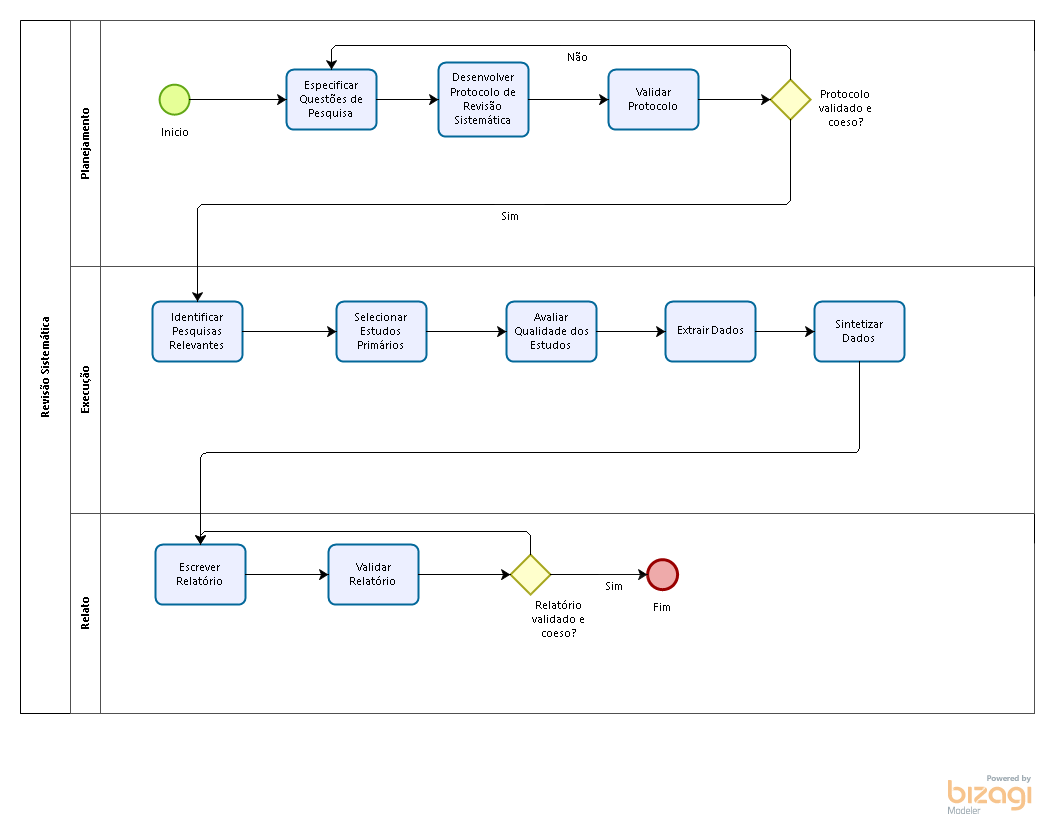
\includegraphics[width=14.5cm]{figuras/revisaoSistematica}
        \caption{Modelagem da Revisão Sistemática}
        Fonte:Autor
		\label{img:processo}
\end{figure}

A Figura \ref{img:processo}, mostrar o processo a ser seguido no desenvolvimento deste artigo.

A fase de planejamento do processo da Figura \ref{img:processo}, possui o objetivo de especificar e validar as questões de pesquisa, desenvolver um protocolo de revisão sistemática e validar o protocolo. A segunda fase, a fase de execução, apresenta as atividades de identificar pesquisas relevantes, selecionar estudos primários, avaliar qualidade de estudos, extrair dados, sintetizar dados. E por último, a fase de relato, tem as atividades de escrever relatório e validar relatório.

\subsection{Objetivos}
\label{subsec:objetivos} 

O objetivo de proposta deste trabalho, utilizando a técnica de Revisão Sistemática de Literatura (RSL), possui a proposta de analisar iniciativas no campo da Inteligência Artificial (IA) que utilizem as memórias artificiais como fator determinante para a tomada de decisões, simulando ações humanas.

A partir do processo da Figura \ref{img:processo}, e levando em consideração o objetivo citado acima, foi elaborado duas questões para direcionar a proposta de pesquisa deste trabalho:

\textbf{Q1}. Como a área da neurociência pode auxiliar pesquisadores de Inteligência Artificial?

\textbf{Q2}. É possível simular ações humanas a partir de memórias artificiais com Inteligência Artificial?

